\section{Surface Geometry}
This section covers the basics introduced in how to represent shapes in a computer.
\subsection{Definitions}
\begin{itemize}
	\item Vertex: A point with three numbers representing its XYZ position in a plane
	\item Edge: An edge is the difference between two vertices; the segment connecting them
	\item Surface: A closed set of edges representing a face of a 3D object
	\item Polygon: A shape in space usually representing by a set of surfaces (other methods listed below)
	\item Polygon Table: 
\end{itemize}
   \begin{figure}[!htb]
	\center{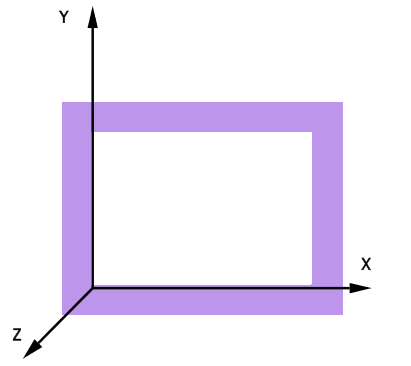
\includegraphics[width=3cm]
		{graphics/rhcoords}}
	\caption{\label{fig:my-label} Coordinate system assumed throughout module}
\end{figure}
When speaking about shapes, we will always assume to be using a right-handed coordinate system. It is named "right-hand" due to the position of the thumb when taking your right hand, placing it on the positive x-axis, the positive z direction will be the direction of the thumb. Right hand just means the thumb is pointed outwards/towards the viewer, so positive z-axis will be towards the viewer.
\newline
\subsection{Examples}
asdads
\subsection{Further Sources}

\newpage
\section{Transforms}
\newpage
\section{Lighting}
\newpage
\section{Projection}
\newpage
\section{Texture Mapping}
\newpage
\section{Past Exam Practice}